\newcommand{\fexpression}{x}
\newcommand{\sexpression}{x+3}
\newcommand{\texpression}{x-2}
\newcommand{\drwdenominator}[1]{
    \ifnum#1=0
    \fexpression(\sexpression)(\texpression)
    \else
    \cancel{\fexpression(\sexpression)(\texpression)}
    \fi
}
\newcommand{\fracexpretion}[1]{
    \ifnum#1=0
    \int\frac{3x+1}{\drwdenominator{#1}}dx
    \else
    \int\frac{3x+1}{\drwdenominator{#1}}dx
    \fi
}
\newcommand{\fraca}[1]{
    \ifnum#1=0
    \frac{1}{6}
    \else
    -\frac{1}{6}
    \fi
}
\newcommand{\fracb}[1]{
    \ifnum#1=0
    \frac{8}{15}
    \else
    -\frac{8}{15}
    \fi
}
\newcommand{\fracc}{\frac{7}{10}}
\newcommand{\drawffraction}{-\frac{\fraca{0}}{x}}
\newcommand{\drawsfraction}{-\frac{\fracb{0}}{x+3}}
\newcommand{\drawtfraction}{+\frac{\fracc}{x-2}}
\newcommand{\drawfexpression}{\fexpression^\fraca{0}}
\newcommand{\drawsexpression}{(\sexpression)^\fracb{0}}
\newcommand{\drawtexpression}{(\texpression)^\fracc}

\textbf{Temática 3 - Integración por Fracciones parciales}
\[\int\frac{3x+1}{x(x^2+x-6)}dx\]
\[
    \begin{aligned}
        Factorizamos: && x(x^2+x-6)
    \end{aligned}
\]
\[\drwdenominator{0}\]
\[\fracexpretion{0}\]
\[\fracexpretion{0}=\frac{A}{\fexpression}+\frac{B}{\sexpression}+\frac{C}{\texpression}\]
\[\fracexpretion{1}=\frac{A(\sexpression)(\texpression)+B\fexpression(\texpression)+C\fexpression(\sexpression)}{\drwdenominator{1}}\]
\[
    \begin{aligned}
        Igualamos && x && a && -3 && para && eliminar && \sexpression
    \end{aligned}
\]
\[-8=15B\]
\[B=\fracb{1}\]
\[
    \begin{aligned}
        Igualamos && x && a && 2 && para && eliminar && \texpression
    \end{aligned}
\]
\[7=10C\]
\[C=\fracc\]
\[
    \begin{aligned}
        Igualamos && x && a && 0 && para && eliminar && \fexpression
    \end{aligned}
\]
\[1=-6A\]
\[A=\fraca{1}\]
\[\fracexpretion{0}=\int\left(\drawffraction\drawsfraction\drawtfraction\right)dx\]
\[
    \begin{aligned}
       \drawffraction && \rightarrow && Factor && linal. \\
       \drawsfraction && \rightarrow && Factor && linal. \\
       \drawtfraction && \rightarrow && Factor && linal.
    \end{aligned}
\]
\[\fracexpretion{0}=\fraca{1}\int\frac{dx}{\fexpression}\fracb{1}\int\frac{dx}{\sexpression}+\fracc\int\frac{dx}{\texpression}\]
\[\fracexpretion{0}=\fracc\ln\left|\texpression\right|\fraca{1}\ln\left|\fexpression\right|\fracb{1}\ln\left|\sexpression\right|+C\]
\[\fracexpretion{0}=\ln\left|\drawtexpression\right|-\ln\left|\drawfexpression\right|-\ln\left|\drawsexpression\right|+C\]
\[\fracexpretion{0}=\ln\left|\frac{\drawtexpression}{\drawfexpression\cdot\drawsexpression}\right|+C\]

\begin{figure}[h]
    \begin{center}
        \fbox{
            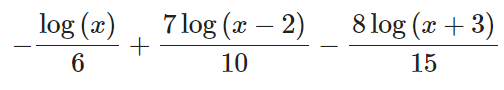
\includegraphics{comp-task3.png}
        }
        \caption{Integración por método de fracciones parciales}
    \end{center}
\end{figure}